\documentclass[a4paper,11pt]{book}
\usepackage[T1]{fontenc}
\usepackage[utf8]{inputenc}
\usepackage{lmodern}

\usepackage{hyperref}
\usepackage{graphicx}
\usepackage[english]{babel}

\title{\Huge \textbf{Genetski algoritmi} \\ \huge Minimizacija funkcije Trogrba kamila \\ }
\author{\textsc{Aleksandar Stojanovic RN97/2018}}


\begin{document}

\frontmatter
\maketitle

\mainmatter

\chapter{Objašnjenje rada}

\section{Jezik i tehnicki detalji}
Za rešavanja datog problema sam se odlučio za python programski jezik zbog lagane obrade podataka. Od biblioteka sam koristio sledeće:

\begin{itemize}
  \item random
  \item sys
  \item decimal
  \item numpy
  \item pprint
  \item configparser - parsiranje fajlova
  \item matplotlib - grafik
\end{itemize}

Instaliranje ovih biblioteka vrši se tako sto iz istog foldera pozovemo sledeću komandu: $pip$ $install$ $-r$ $requirements.txt$ \\
Za pokretanje programa neophodno je sve fajlove staviti u isti folder.\\

Struktura fajlova je sledeća:
\begin{itemize}
  \item config.properties
  \item output.txt
  \item main.py
\end{itemize}

U $config.properties$ fajlu se nalaze default vrednosti koje ce algoritam koristiti ukoliko korisnik ne unese svoj fajl. Nakon sto algoritam završi sa radom u folderu će biti kreiran fajl koji sadrži rezultate pokretanja sa nazivom $output.txt$.

\section{Algoritma}
Korišćen je kontinualan genetski algoritam. Ovaj algoritam sadrži sledeće komponente:

\begin{itemize}
  \item Funkcija prilagodjenosti,
  \item funkcija ukrštanja i
  \item funkcija mutacije. 
\end{itemize}

One će biti objasnjene kasnije u posebnim sekcijama, za sada ću se fokusirati na parametre.\\

U folderu se nalazi $config.properties$ fajl koji sadrzi polja za konfiguraciju algoritma. Pri pokretanju programa, od korisnika ce biti zatraženo da unese putanju do fajla za konfiguraciju. Ukoliko korisnik ne unese fajl, program će ucitati vrednosti iz ovog fajla. \\

Ako pogledamo sastav fajla možemo primetiti dva poglavlja. Poglavlje $population$ odnosi se na konfiguraciju se populacije i ovde se može podesiti:

\begin{itemize}
  \item Veličina populacije (3 polja jer nemam skilla),
  \item Donja granica intervala,
  \item Goranja granica intervala,
  \item Koeficijent koji odredjuje mutaciju i 
  \item Velicina test objekta.
\end{itemize}
 
Pogravlje $general$ sadrži polja za konfiguraciju algoritma:
\begin{itemize}
  \item Maksimalnog broja iteracija,
  \item Lokaciju output fajla,
  \item Broj ponavljanja po velicini populacije,
  \item Prikaz grafika i
  \item Cuvnaje grafika u $.png$ obliku
\end{itemize} 

\section{Metoda prilagodjenosti}

Funkcija prilagodjenisti predstavlja način za rangiranje populacije uz pomoc fitness-a. Budući da mi radimo minimizaciju visedimenzionalne funkcije možemo nju koristiti kao funkciju troška. Ovo u prevodu znaci da konkretno u našem slučaju hromozomi imaju u sebi dva gena $[x,y]$ koje ubacujemo u funkciju. Njihov fitnes je zapravo vrednost funkcije za parametre koje smo prosledili.\\

Nama je poznat interval za koji funkcija radi i znamo da se očekivana nula nalazi u $f(0,0)=0$. Sa ovim možemo rangirati jedinke tako što ćemo na osnovu fitnesa sortirati populaciju u rastućem poretku. Jedinke koje su bliže nuli će imati najveći fitnes.

\section{Metoda ukrštanja - Redklif ukrštanje}

Za metodu ukrštanja koristio sam Redklifovo jednostavno ukrštanje. U jednom od svojih radova Redklif je predložio jednostavnu formulu za izračunavanje vrednosti jednog parametra potomka iz vrednosti istog parametara kod njegova dva roditelja. Ova formula izgleda ovako:
\[\rho_{pot} = \beta * \rho_{1} + (1-\beta) * \rho_{2}\]

U ovoj formuli $\rho_{pot}$ predstavlja parametar poromka, $\rho_{1}$ i $\rho_{2}$ su parametri prvog i drugog roditelja. $\beta$ je slučajan broj kojim se odredjuje udeo vrednosti parametra prvog i drugog roditelja u brednost parametra dobijenog potomka. Ovo se postiže tako sto je $\beta$ fiksiran izmedju vrednosti $[0,1]$. Kada je $\beta=0$, vrednost parametra se prepisuje od drugog roditelja, kada je $\beta=1$, vrednost se uzima od prvog roditelja, a kada je $\beta=0.5$, vrednost je aritmetička sredina vrednosti parametra oba roditelja.

\section{Metoda mutacije - Tačkasta normalna mutacija}

Jednostavna metoda kod koje se na gen iz normalne raspodele dodaje slucajna vrednost. Bilo bi lepo definisati optimalan interval iz kojeg cemo birati istu radi bržeg konvergiranja ka cilju ali ja sam se odlučio za vrednosti izmedju 0 i 1.

\chapter{Izvršavanje}

\section{Grafik}

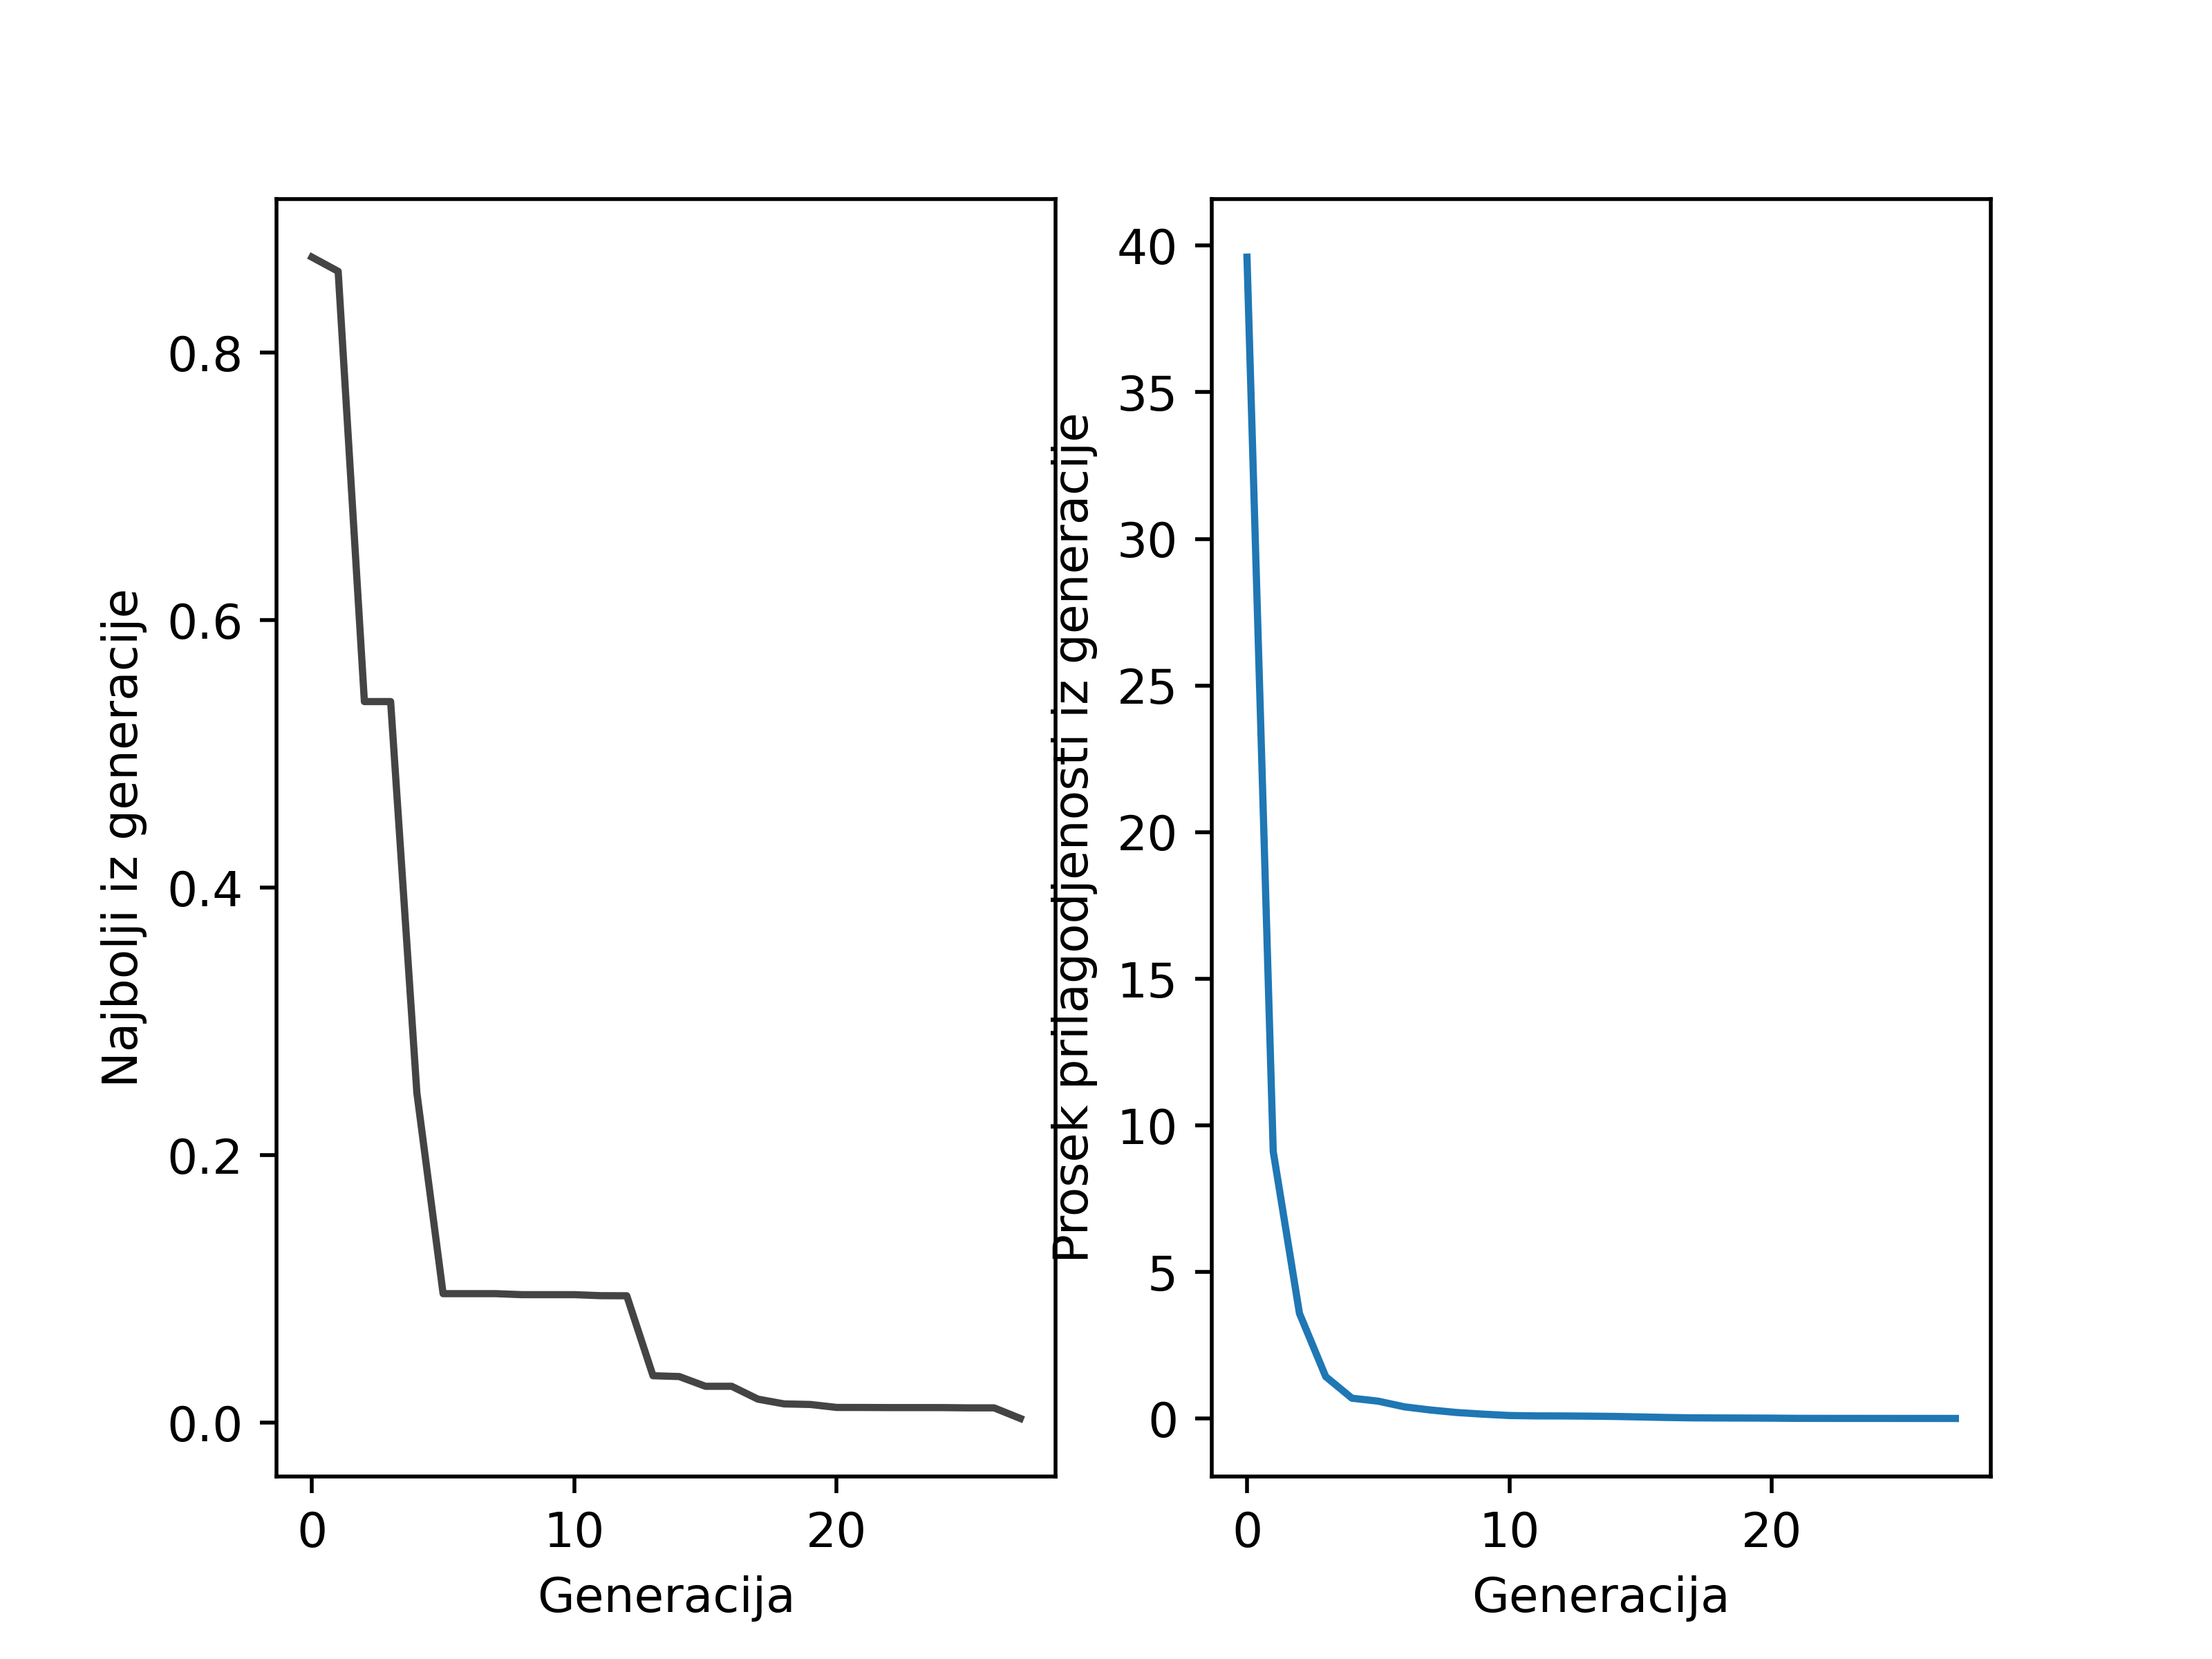
\includegraphics{grafik20-0.png}

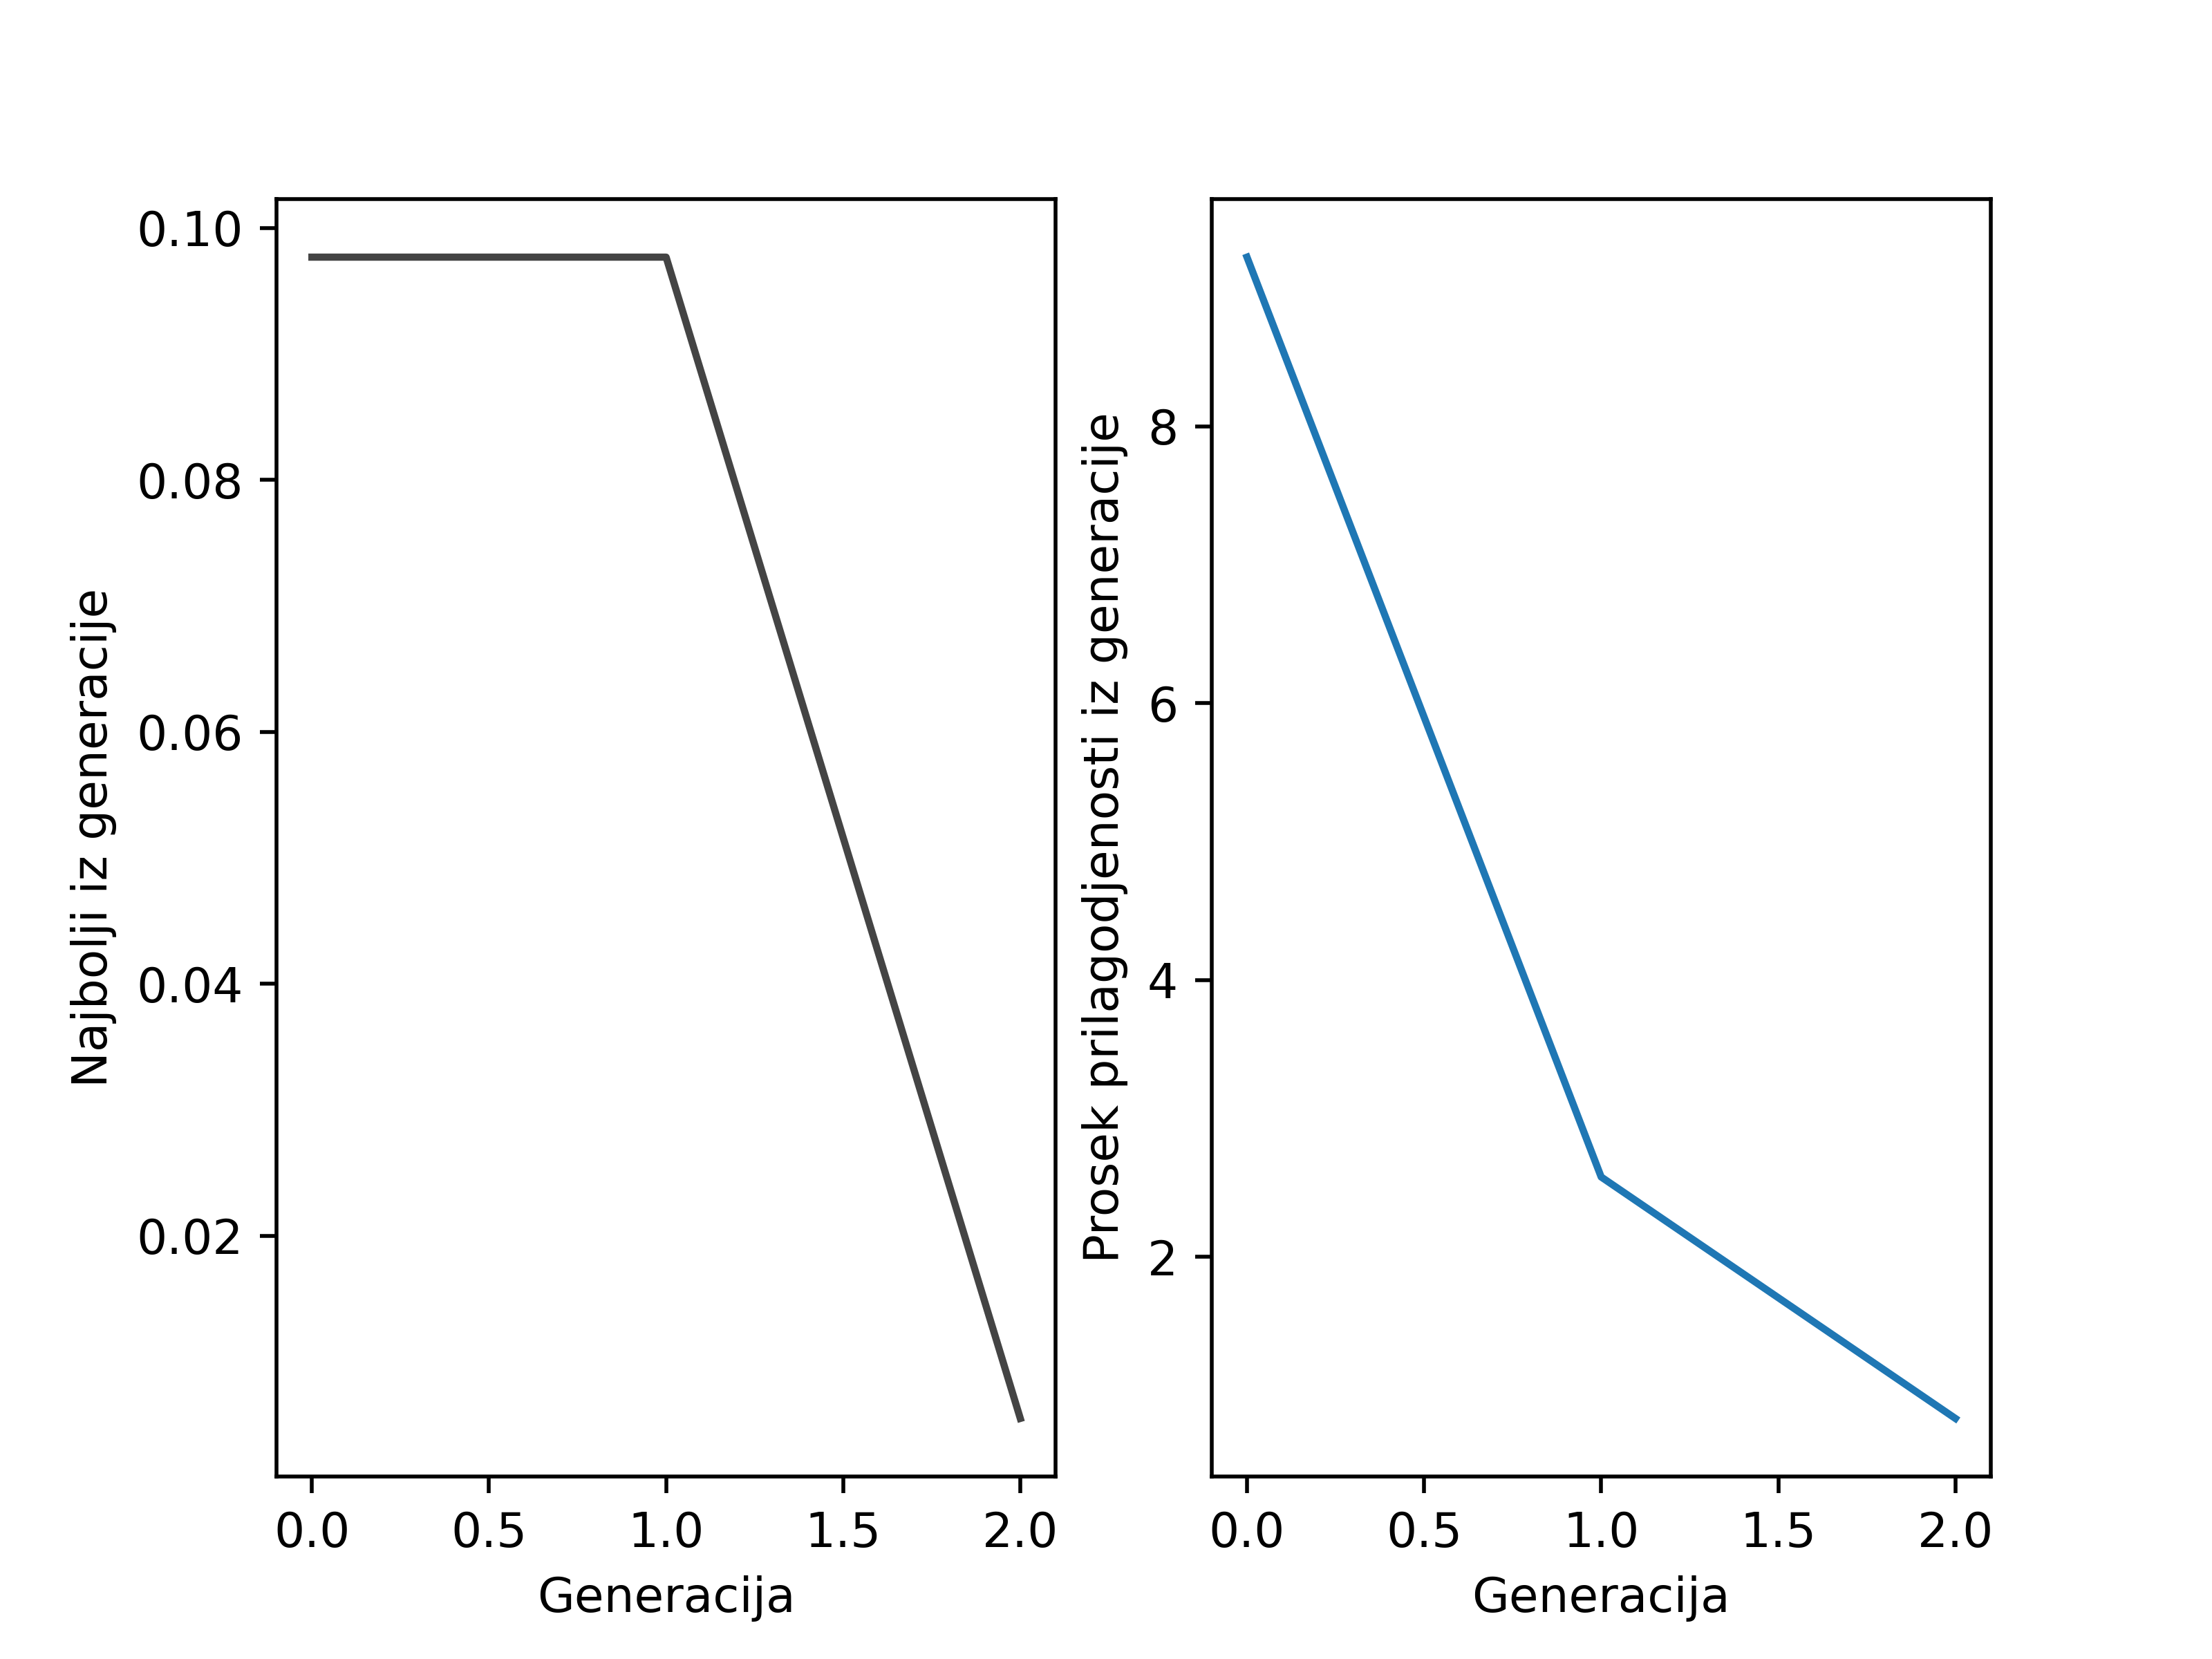
\includegraphics{grafik100-0.png}

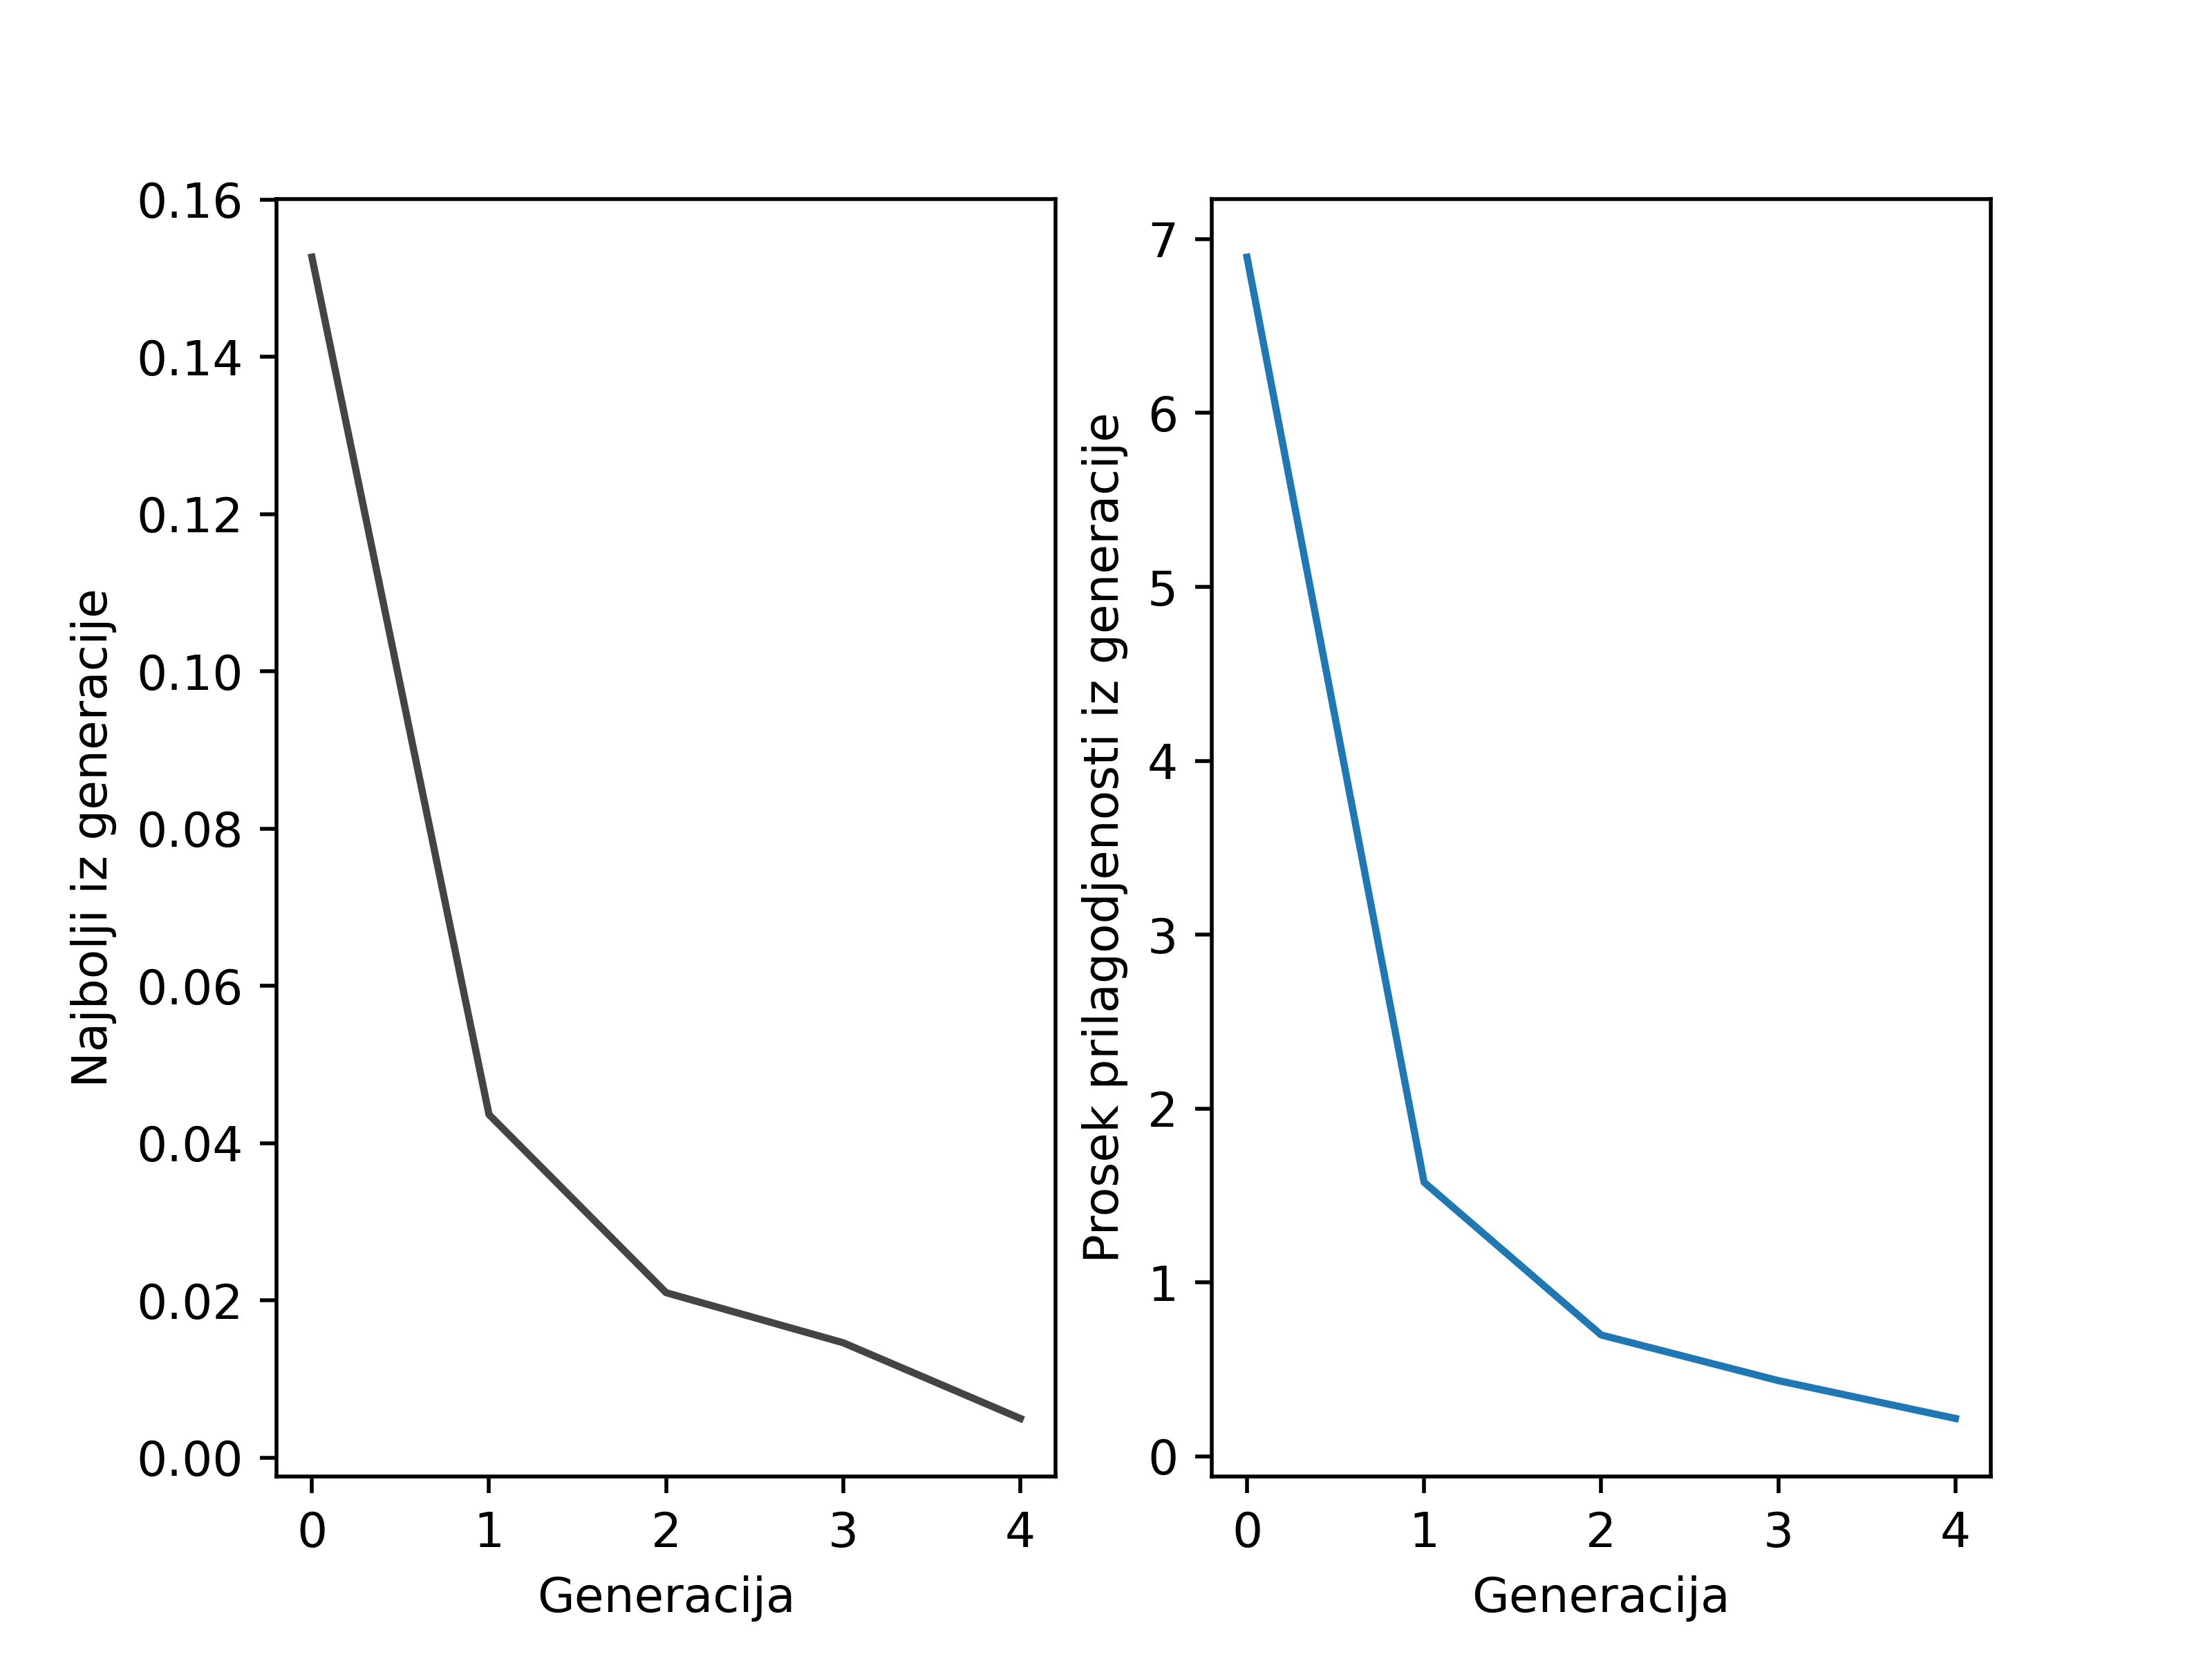
\includegraphics{grafik150-0.png}
\end{document}